\documentclass[12pt,a4paper,twoside]{article}
\usepackage{geometry}
\geometry{a4paper}

\usepackage[utf8]{inputenc} %kompilowanie polskich literek
\usepackage[OT1]{fontenc} %wyświetlanie polskich literek
\usepackage{polski} %wyświetlanie polskich literek cz. II
\usepackage[english,polish]{babel} %zasady łamania wierszy, domyślnie polski
\usepackage{hyperref} %możliwość linkowania
\usepackage{graphicx} %wstawianie obrazków
\usepackage{epstopdf} %wstawianie obrazków w formacie .eps
\usepackage{multicol} %środowisko dwukolumnowe
\usepackage{capt-of} %\captionof
\usepackage{units} %\nicefrac

\begin{document}

\newcommand{\en}[1]{\textit{\enn{#1}}}
\newcommand{\enn}[1]{\foreignlanguage{english}{#1}}
\newcommand{\renmich}[1]{\textbullet{}\marginpar{\tiny \raggedright renmich{}: #1}}

\begin{titlepage}
    \begin{center}

    \vspace{1cm}
    {\Huge Dokumentacja projektu magisterskiego} \\[0.5cm]
    {\Large Marcin Kurczewski}
    \end{center}

    \vspace{3cm}
    \hspace{8cm}\parbox[l]{6cm}{\Large Praca magisterska \\
    napisana pod kierunkiem \\
    dr Michała Rena}

    \begin{center}
    \vspace{4cm}
    Poznań, \today
    \end{center}
\end{titlepage}

\section{Założenia projektu}

Projekt ma za zadanie przeprowadzić \en{collision attack} na kryptograficzne
funkcje skrótu \texttt{MD4} oraz \texttt{MD5}, tj. znaleźć dwie wiadomości
$m_1, m_2 : m_1 \neq m_2$ takie, że $\mathtt{MD4}(m_1) = \mathtt{MD4}(m_2)$
w~wariancie \texttt{MD4} lub $\mathtt{MD5}(m_1) = \mathtt{MD5}(m_2)$
w~wariancie \texttt{MD5}. W~tym celu powstały dwie wersje projektu: pierwsza~--
\texttt{md4coll}~-- znajduje kolizje dla \texttt{MD4}, druga~--
\texttt{md5coll}~-- dla \texttt{MD5}.

\section{Zarys projektu}

\subsection{Historia}

W~roku~2004 na spotkaniu CRYPTO Xiaoyun Wang zaprezentowała parę wiadomości
dającą taki sam skrót \texttt{MD4} oraz parę wiadomości dającą taki sam skrót
\texttt{MD5}, jednak algorytm, którym się posłużyła nie został wówczas
opublikowany~\cite{wang2004finding}. Philip Hawkes dokonał szczegółowej analizy
wiadomości i~ich skrótu \texttt{MD5}~\cite{hawkes2004musings}, lecz nie udało
mu się rzucić światła na algorytm wyszukujący wiadomości. Rok później Vlastimil
Klima znalazł algorytm wyszukujący kolizje
\texttt{MD5}~\cite{klima2005finding1}, lecz zamiast go opublikować, podał tylko
niepotwierdzalne statystyki dotyczące szybkości działania oraz~opublikował
przykładowe kolizje. Algorytm miał działać dużo
szybciej~\cite{klima2006tunnels} od oryginalnego algorytmu użytego przez Wang.
Wreszcie, tego samego roku Wang opublikowała użyty przez siebie algorytm do
łamania \texttt{MD4}~\cite{wang2005md4} oraz \texttt{MD5}~\cite{wang2005md5} na
konferencji EUROCRYPT. Wykazano jednak później, że atak na~\texttt{MD5} jest
nieoptymalny~\cite{klima2005finding2,klima2006tunnels}, a~sama praca zawiera
drobne błędy~\cite{yajima2005wang,sasaki2005improved,liang2007improved}.
Podobnie ma się sprawa z~\texttt{MD4}~\cite{naito2005improved}.

\subsection{Prace źródłowe}

Oba ataki opierają się w~głównej mierze na pracach Xiaoyun Wang~--
\cite{wang2005md4} w~przypadku \texttt{MD4} oraz \cite{wang2005md5} w~przypadku
\texttt{MD5}. Dodatkowo atak na \texttt{MD5} jest usprawniony rezultatami
z~prac~\cite{yajima2005wang,sasaki2005improved,liang2007improved} w~celu
poprawienia tzw. warunków wystarczających oraz z~\cite{klima2005finding2} w~celu
zmniejszenia złożoności obliczeniowej ataku. Techniki modyfikacji wiadomości są
luźno inspirowane\renmich{nieco zbyt kolokwialnie} inną implementacją ataku na \texttt{MD4}~\cite{stach2005md4}
i~\texttt{MD5}~\cite{stach2005md5}.

\subsection{Wcześniejsze rezultaty}

Jedyną znaną implementacją ataku na \texttt{MD4} oraz \texttt{MD5} są programy
Patricka Stacha~\cite{stach2005md4,stach2005md5}. Działają one szybko, lecz
implementacja ataku na \texttt{MD5} zawiera drobny błąd, który został
poprawiony w~tym projekcie. Ponadto techniki modyfikacji wiadomości użyte
w~implementacji Patricka\renmich{Tak po imieniu?} nie są optymalne.

\section{Implementacja ataku na \texttt{MD4}}

Poniżej został opisany ogólny schemat ataku na \texttt{MD4} użyty w~projekcie.

\begin{enumerate}

\item Weź wiadomość $m_0$ składającą się z~1 bloku (512 bitów).

\item Weź wiadomość $m_1 = m_0 + \Delta$, gdzie $\Delta$ jest pewną stałą.

\item Równolegle zacznij liczyć $\mathtt{MD4}(m_0)$ oraz $\mathtt{MD4}(m_1)$,
tj. wykonuj kolejne operacje \texttt{MD4}, niezależnie pamiętając kolejne
wartości stanu wewnętrznego dla obu wiadomości.

\item Po każdej operacji sprawdź, czy spełnione zostały warunki wystarczające.
Warunki wystarczające to warunki narzucone na stan wewnętrzny funkcji skrótu,
różnice między stanami wewnętrznymi dla $m_0$ i~$m_1$ oraz wreszcie różnice
między $m_0$ i~$m_1$ ($m_0 \stackrel{?}{=} m_1 + \Delta$). Gdy dla wszystkich
operacji \texttt{MD4} wszystkie warunki wystarczające są spełnione, atakujący
może mieć pewność że $H(m_0) = H(m_1)$.

\item Jeżeli warunki nie zostały spełnione, spróbuj~-- jeżeli jest to
możliwe~-- zmodyfikować $m_0$ i~$m_1$ w~odpowiedni sposób, wyliczyć nowe
wartości stanów wewnętrznych i~ponownie sprawdzić, czy zostały spełnione
warunki wystarczające. Jeżeli to nie pomoże, ponów procedurę dla innej pary
wiadomości.

\end{enumerate}

Zarówno warunki wystarczające, jak i~$\Delta$ użyte w~projekcie zostały
bezpośrednio zaczerpnięte z~\cite{wang2005md4}. Praca nie opisuje w~jaki sposób
dojść do tych warunków; podejrzewa się, że zostały one odkryte na podstawie
ręcznej analizy. Przypuszcza się, że istnieją inne $\Delta$, dla których można
sformułować mniej warunków wystarczających (a~zatem zmniejszyć złożoność
obliczeniową ataku), lecz w~praktyce nikt nie próbował zajmować się innymi
$\Delta$ niż zostało to zaproponowane w~\cite{wang2005md4}.

Ponieważ warunków wystarczających jest wiele, szansa, że wszystkie zostaną
spełnione jest bardzo niewielka~-- mniejsza nawet od szansy na znalezienie
kolizji na podstawie paradoksu urodzinowego. Dlatego krok, w~którym dokonujemy
modyfikacji $m_0$ i~$m_1$ próbując zapewnić spełnienie tych warunków jest
krytycznie ważny.

Jednym z~najważniejszych spostrzeżeń jest fakt, że w~pierwszej rundzie każdy
bit wiadomości wpływa co najwyżej na jeden bit stanu wewnętrznego. Pozwala to
nam na optymalizację ataku: zamiast brać przypadkowe $m_0$ i~$m_1$, możemy
wziąć przypadkową serię stanów wewnętrznych, które powstałyby na skutek
wykonania pierwszej rundy, następnie zapewnić prostymi operacjami bitowymi,
żeby spełniły warunki wystarczające i~na końcu je odwrócić, otrzymując $m_0$
i~$m_1$. (Otrzymanie $m_0$ i~$m_1$ na podstawie stanów wewnętrznych z~rundy
pierwszej jest możliwe poprzez odwrócenie procedury \texttt{MD4}, wyliczającej
stan wewnętrzny na podstawie $m_0$ i~$m_1$.) Procedura ta została nazwana
\en{Simple Message Modification} i~gwarantuje, że po pierwszej rundzie
$\mathtt{MD4}_{R1}(m_0) = \mathtt{MD4}_{R1}(m_1)$.

Sytuacja komplikuje się, gdy obliczana jest druga oraz trzecia runda
\texttt{MD4}. Wówczas bity $m_0$ i~$m_1$ zaczynają być wykorzystywane do
aktualizacji stanu wewnętrznego po raz drugi i~trzeci, lecz tym razem w~całkiem
innych miejscach. Mimo\renmich{przecinek?} że większość warunków wystarczających dotyczy tylko
pierwszej rundy, to liczba warunków dla stanu wewnętrznego w~rundzie drugiej
i~trzeciej nie pozostaje\renmich{jest? ,,pozostaje'' sugeruje, że coś się dzieje w pierwszej rundzie i wpływa na liczbę warunków} mała,\renmich{kropka?} stąd aby zapewnić kolizje także w~późniejszych
fazach wprowadza się tzw. \en{Advanced Message Modification}.

Wang zaproponowała skomplikowane techniki korekcji pojedynczych warunków
w~późniejszych rundach, opierające się na aktualizacji bitów $m_0$ i~$m_1$
zależnie od okoliczności (przy niespełnieniu danego warunku, użyj
odpowiadającej mu techniki modyfikacji $m_0$ i~$m_1$)~\cite{wang2005md4}.
Podejście to jest jednak trudne w~implementacji; do tego samego wniosku doszedł
także Patrick Stach w~swojej implementacji ataku Wang~\cite{stach2005md4}.
Stach zamiast wybierać ręcznie bity i~sprawdzać różne warunki, po prostu losuje
stan wewnętrzny dla operacji $i \geq 17$ (czyli dla rund późniejszych niż~1)
i~aktualizuje te słowa wiadomości, które wpływają na dany stan, po czym oblicza
z~powrotem wszystkie stany \texttt{MD4}, które mogły się zmienić na skutek
modyfikacji $m_0$ i~$m_1$. Na końcu sprawdza spełnienie warunków
wystarczających. Podejście to przyjął również autor tego projektu.

\section{Implementacja ataku na \texttt{MD5}}

Różnice między \texttt{MD4} i~\texttt{MD5} w~praktyce sprowadzają się do
zwiększenia liczby rund z~3 do~4~oraz wprowadzeniu dodatkowej operacji
\texttt{XOR} wykonywanej po cyklicznym przesunięciu bitowym:
\renmich{Jeśli rysunki miały być obok siebie, to nie wyszło. Co więcej, wykraczają poza dolny margines strony\ldots}
\begin{multicols}{2}
\begingroup
    \centering
    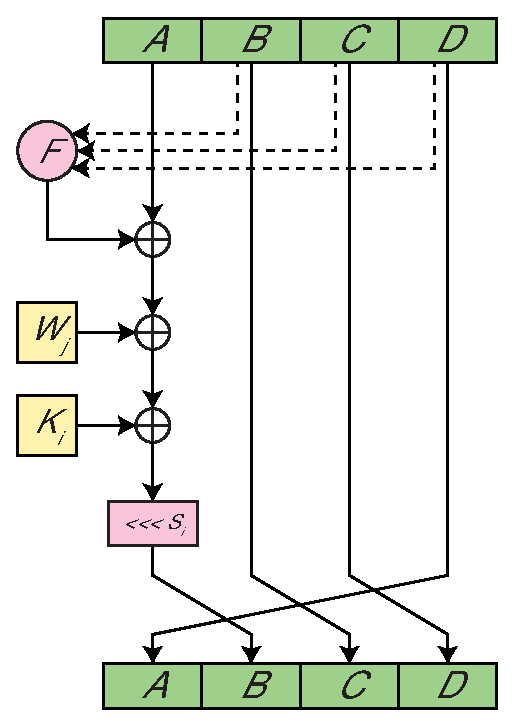
\includegraphics[width=6cm]{img/md4_operation.eps}
    \captionof{figure}{Jedna operacja \texttt{MD4}}
    \label{fig:md4_operation}
\endgroup

\begingroup
    \centering
    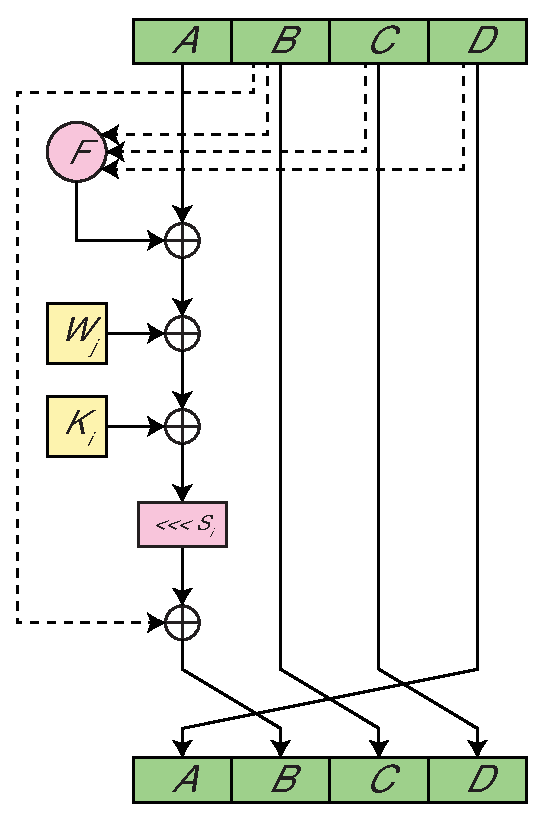
\includegraphics[width=6cm]{img/md5_operation.eps}
    \captionof{figure}{Jedna operacja \texttt{MD5}}
    \label{fig:md5_operation}
\endgroup
\end{multicols}


Atak na \texttt{MD5} przebiega bardzo podobnie jak atak\renmich{do ataku} na \texttt{MD4}. Jednak
opisane wyżej różnice wystarczają, aby prawdopodobieństwo spełnienia warunków
wystarczających, nawet po zastosowaniu \en{Advanced Message Modification}, było
dużo mniejsze. W~przypadku ataku na \texttt{MD4} kolizje zostały wyszukiwane
wśród par wiadomości składających się z~jednego bloku; w~przypadku \texttt{MD5}
sprawdzane są wiadomości składające się z~dwóch bloków. Oznacza to, że po
obliczeniu \texttt{MD5} dla bloku pierwszego oczekujemy pewnej różnicy między
$\mathtt{MD5}(m_{0,B1})$ a~$\mathtt{MD5}(m_{1,B1})$; później ta różnica jest
korygowana poprzez modyfikacje $m_{0,B2}$ oraz $m_{1,B2}$.

Ponieważ prawdopodobieństwo znalezienia dobrej wiadomości jest dużo mniejsze,
ważny jest dobór dobrych warunków wystarczających oraz technik modyfikacji
wiadomości. Program Patricka Stacha~\cite{stach2005md5}, który
implementuje~\cite{wang2005md5}, zawiera drobny błąd w~warunkach
wystarczających; ponadto nie uwzględnia poprawek zaproponowanych w~późniejszych
pracach. Autor projektu uwzględnił poprawki
z~\cite{yajima2005wang,sasaki2005improved,liang2007improved} oraz dodał
brakujący warunek z~\cite{wang2005md5} (dokładnie: warunek $c_{1,12} = 0$).
Techniki \en{Advanced Message Modification} implementują propozycje
przedstawione przez Vlastimila Klimę~\cite{klima2005finding2}.

\section{Możliwe usprawnienia}

\renmich{\ldots{}A możliwe usprawnienie to\ldots{}? Uruchomienie na szybszym komputerze? Czegoś chyba brakuje.}Na komputerze wyposażonym w~procesor i5~750 i~4GB RAM-u, znalezienie kolizji
\texttt{MD4} zajmuje około 4\nicefrac{1}{2}~sekund; znalezienie kolizji
\texttt{MD5} zajmuje około 2\nicefrac{1}{4} godziny. 

\newpage
\bibliographystyle{plain}
\bibliography{bibliography}

\end{document}
